

\chapter{Results}

In this chapter, we describe the results from our pose and depth experiments. In Chapter 3 we described an unsupervised pipeline for learning depth and visual odometry from monocular imagery. Similarly, in Chapter 4 we adapted conventional 2D machine learning techniques to apply 4D image data to learning these tasks. Specifically, we recommended two variants of an algorithm for learning depth and visual odometry from light fields - the first uses all the information from the light field to generate a novel rendering of a single \textit{U, V} slice, while the second method uses the known configuration of the camera array to create a rendering of the complete light field. In this chapter, we contrast results for three algorithms - each of the two novel pipelines described in Chapter 4, and the existing monocular approach described in Chapter 3. For the two algorithms that we have suggested, we also evaluate three ingestion methods: focal-stacks, volumetric images, and tiled EPI images. 

First, we evaluate each algorithm's performance in pose-estimation, and demonstrate results for cumulated trajectories for several input-sequences. Subsequently, we'll evaluate the algorithms' performance in depth-prediction and photometric reconstruction. 


\section{Experimental Setup Details}
In each of our experiments, we use the same training dataset of 9000 grayscale input images consisting of 48 short video-sequences. The testing set, which is also the same across all experiments, consists of ~400 input images over 4 video-sequences. For training we use a batch size of 2 images, and train for a total of 300 epochs. 


\section{Pose Estimation and Visual Odometry}

An important metric of error that we use to evaluate pose prediction, is the \textit{absolute instantaneous error} for each of the 6 degrees-of-freedom that are estimated. This metric describes the magnitude of the error between the predicted and the true component. As described in Chapter 4, we have collected ground-truth pose data using a robotic manipulator platform with a repeatability of $\pm 0.01$ millimeters, thus allowing a strong evaluation of pose-estimation. Meanwhile, we can evaluate each pipeline's effectiveness in estimating the \textit{average cumulative error} by comparing the true trajectory with the predicted trajectory. 


\subsection{Single-view Reconstruction Approach}

The following histograms summarise 400 observations of the absolute instantaneous error for each of the 6 degrees of freedom (translation and rotation in X, Y and Z), over three input methods (tiled epipolar images, focal stacks, and volumetric stacks).

\begin{figure}[H]
    \centering
    \includegraphics[width=\textwidth, height=3.35in]{images/result-examples/pose/errors/singlewarp-epi.png}
    \caption{Instantaneous absolute errors when \textbf{tiled epipolar images} are the input method.}
\end{figure}

\begin{figure}[H]
    \centering
    \includegraphics[width=\textwidth, height=3.35in]{images/result-examples/pose/errors/singlewarp-focalstack-17-5.png}
    \caption{Instantaneous absolute errors when \textbf{focal stacks} images are the input method.}
\end{figure}

\begin{figure}[H]
    \centering
    \includegraphics[width=\textwidth, height=3.35in]{images/result-examples/pose/errors/singlewarp-stack.png}
    \caption{Instantaneous absolute errors when \textbf{volumetric stacks} are the input method.}
\end{figure}

Figure 5.5 shows 2 examples of true and estimated trajectories for the three input methods. 

\begin{figure}[H]
    \subfloat[Tiled EPIs]{
        \includegraphics[height=1.9in]{images/result-examples/pose/trajectories/singlewarp/sw-epi-16.png}
    }
    \subfloat[Focal Stacks]{
        \includegraphics[height=1.9in]{images/result-examples/pose/trajectories/singlewarp/sw-focalstack-175-16.png}
    }
    \subfloat[Volumetric Images]{
        \includegraphics[height=1.9in]{images/result-examples/pose/trajectories/singlewarp/sw-stack-16.png}
    }\\
    \caption{Estimated and true trajectories for input sequence 16.}
    \setcounter{subfigure}{0}

    \subfloat[Tiled EPIs]{
        \includegraphics[height=1.9in]{images/result-examples/pose/trajectories/singlewarp/sw-epi-44.png}
    }
    \subfloat[Focal Stacks]{
        \includegraphics[height=1.9in]{images/result-examples/pose/trajectories/singlewarp/sw-focalstack-175-44.png}
    }
    \subfloat[Volumetric Images]{
        \includegraphics[height=1.9in]{images/result-examples/pose/trajectories/singlewarp/sw-stack-44.png}
    }
    \caption{Estimated and true trajectories for input sequence 44.}
    \setcounter{subfigure}{0}
\end{figure}

Table 5.1 summarises the instantaneous and cumulative errors for the three input methods. 
 
\begin{table}[htbp]
    \caption{Mean Absolute Instantaneous Error and Cumulative Error}
    \centering
    \begin{tabular}{@{}lll@{}}
        \toprule
        Input Method        & Absolute Instantaneous Error (mm)   & Cumulative Error (mm) \\
        \midrule 
        Tiled EPI Polar Images & \textbf{9.64} & \textbf{71.38} \\
        Focal Stacks & 9.79 & 104.03 \\
        Volumetric Stacks & 12.17 & 103.47 \\
        \bottomrule
        
    \end{tabular}
\end{table}


\subsection{Light field Reconstruction Appraoch}

Here we describe the performance of the second variant of our suggested pipeline, using the known camera configuration to photometrically warp the complete light field. Because this pipeline incorporates known information about the relationship between individual sub-apertures on the camera module, we expect this pipeline to demonstrate improved performance in pose estimation and scale-awareness.

We carry this expectation because this variant of the pipeline generates a stronger supervision signal - the larger number of pixels being warped results in a significantly heavier loss for the same error, compared with the single-view reconstruction approach. Additionally, this variant carries a much smaller tolerance to scale inconsistencies due to the constraints imposed when incorporating multiple sub-apertures and their known relative spacing.


\begin{figure}[H]
    \centering
    \includegraphics[width=\textwidth, height=3.2in]{images/result-examples/pose/errors/multiwarp-epi.png}
    \caption{Instantaneous absolute errors when \textbf{tiled epipolar images} are the input method.}
\end{figure}
\begin{figure}[H]
    \centering
    \includegraphics[width=\textwidth, height=3.2in]{images/result-examples/pose/errors/multiwarp-focalstack-17-5.png}
    \caption{Instantaneous absolute errors when \textbf{focal stacks} are the input method.}
\end{figure}
\begin{figure}[H]
    \centering
    \includegraphics[width=\textwidth, height=3.2in]{images/result-examples/pose/errors/multiwarp-stack.png}
    \caption{Instantaneous absolute errors when \textbf{volumetric stacks} are the input method.}
\end{figure}



\begin{figure}[H]
    \subfloat[Tiled EPIs]{
        \includegraphics[height=2in]{images/result-examples/pose/trajectories/multiwarp/mw-epi-16.png}
    }
    \subfloat[Focal Stacks]{
        \includegraphics[height=2in]{images/result-examples/pose/trajectories/multiwarp/mw-fs-175-16.png}
    }
    \subfloat[Volumetric Images]{
        \includegraphics[height=2in]{images/result-examples/pose/trajectories/multiwarp/mw-stack-16.png}
    }
    \caption{Estimated and true trajectories for input sequence 16.}
    \setcounter{subfigure}{0}
    \subfloat[Tiled EPIs]{
        \includegraphics[height=2in]{images/result-examples/pose/trajectories/multiwarp/mw-epi-44.png}
    }
    \subfloat[Focal Stacks]{
        \includegraphics[height=2in]{images/result-examples/pose/trajectories/multiwarp/mw-fs-175-44.png}
    }
    \subfloat[Volumetric Images]{
        \includegraphics[height=2in]{images/result-examples/pose/trajectories/multiwarp/mw-stack-44.png}
    }
    \caption{Estimated and true trajectories for input sequence 44.}
    \setcounter{subfigure}{0}
\end{figure}

\begin{table}[htbp]
    \caption{Mean Absolute Instantaneous Error and Cumulative Error}
    \centering
    \begin{tabular}{@{}lll@{}}
        \toprule
        Input Method        & Absolute Instantaneous Error (mm)  & Cumulative Error (mm)  \\
        \midrule 
        Tiled EPI Polar Images & \textbf{7.61} & \textbf{50.61} \\
        Focal Stacks & 9.71 & 73.40 \\
        Volumetric Stacks & 10.50 & 110.04 \\
        \bottomrule
        
    \end{tabular}
\end{table}


\subsection{Monocular Approach}

Importantly, we compare our results to the monocular approach using the algorithm suggested by \cite{zhou2017unsupervised}. In this instance, the pair of convolutional networks are not exposed to any sort of light field imagery - the input image is a single 2D image and the photometric warp is similarly performed on a single 2D image. 

\begin{figure}[H]
    \centering
    \includegraphics[width=\textwidth, height=3in]{images/result-examples/pose/errors/singlewarp-stack.png}
    \caption{Instantaneous absolute errors when using \textbf{monocular imagery}.}
\end{figure}

\begin{figure}[H]
    \centering
    \subfloat[Sequence 16]{
        \includegraphics[height=2.1in]{images/result-examples/pose/trajectories/monocular/monocular-16.png}
    }
    \subfloat[Sequence 44]{
        \includegraphics[height=2.1in]{images/result-examples/pose/trajectories/monocular/monocular-44.png}
    }
    \caption{Estimated and true trajectories using monocular imagery.}
    \setcounter{subfigure}{0}
\end{figure}



\subsection{Comparison between Approaches and Summary}

\begin{figure}[H]
    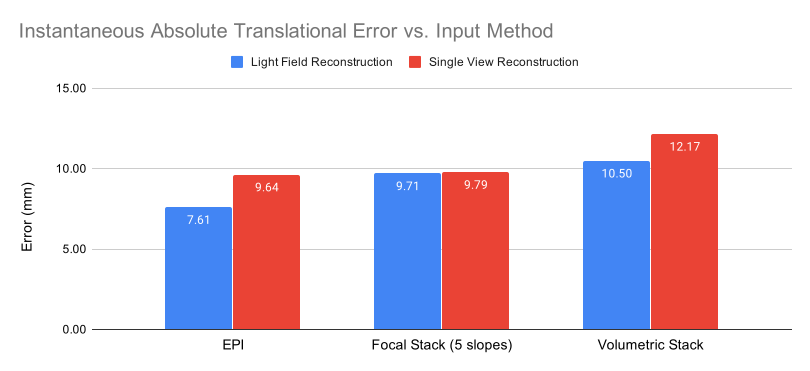
\includegraphics[width=\textwidth]{images/result-examples/bargraphs/iate-vs-inputmethod.pdf}
    \caption[Instantaneous translational errors vs. input methods.]{We find that in terms of translational error, the light field reconstruction pipeline has an edge over the single-view warp variant in all three cases. Additionally, using tiled EPI's demonstrates the smallest translational error of the three input methods.}
\end{figure}
\begin{figure}[H]
    \includegraphics[width=\textwidth]{images/result-examples/bargraphs/cte-vs-inputmethod.pdf}
    \caption[Cumulative translational errors vs. input methods.]{Similarly, we find that over the course of an entire video-sequence, tiled EPI's once again outperform all other input strategies. Over an entire video-sequence, the light field reconstruction pipeline generally outperforms the single-warp pipeline.}
\end{figure}
\begin{figure}[H]
    \includegraphics[width=\textwidth]{images/result-examples/bargraphs/iare-vs-input-method.pdf}
    \caption{We find that in rotational terms, light-field-reconstruction far outperforms the single-view-reconstruction pipeline. Similarly, we find that once again, the tiled EPI insertion strategy demonstrates the smallest error in terms of rotation on our validation dataset.}
\end{figure}
\section{Depth and Photometric Reconstruction}

Aside from pose predictions and trajectories, our pipeline also generates depth-map predictions. In this section, we evaluate these outputs. Because our data acquisition did not include the collection of ground-truth depth data, we must find more creative ways of evaluating depth. One way we can do this is by inspecting the visual quality of the depth maps, observing the artifacts and details resolved. For example, in the depth maps shown, we include a particularly challenging scenario that includes a wire-frame model of a flamingo. 

Another way we can evaluate the quality of our depth maps is to compare the photometric loss from image synthesis. Comparing the synthesised image with the ground-truth image, we can compute a difference-image which shows the magnitude of the error in rendering the synthesised image.


\subsection{Single-view Reconstruction Approach}
\begin{figure}[H]
    \centering
    \subfloat[Input Image]{
        \includegraphics[height=0in, width=1.4in]{images/blank.png}
    }
    \subfloat[Volumetric Stack]{
        \includegraphics[height=0in, width=1.4in]{images/blank.png}
    }
    \subfloat[Focal Stack]{
        \includegraphics[height=0in, width=1.4in]{images/blank.png}
    }
    \subfloat[Tiled EPIs]{
        \includegraphics[height=0in, width=1.4in]{images/blank.png}
    }\\ 
    \subfloat{
        \includegraphics[height=1in]{images/result-examples/depth/16-18.png}
    }
    \subfloat{
        \includegraphics[height=1in]{images/result-examples/depth/singlewarp/stack/16-18.png}
    }
    \subfloat{
        \includegraphics[height=1in]{images/result-examples/depth/singlewarp/focalstack-17-5/16-18.png}
    }
    \subfloat{
        \includegraphics[height=1in]{images/result-examples/depth/singlewarp/epi/16-18.png}
    }\\ 
    \subfloat{
        \includegraphics[height=1in]{images/result-examples/depth/16-50.png}
    }
    \subfloat{
        \includegraphics[height=1in]{images/result-examples/depth/singlewarp/stack/16-50.png}
    }
    \subfloat{
        \includegraphics[height=1in]{images/result-examples/depth/singlewarp/focalstack-17-5/16-50.png}
    }
    \subfloat{
        \includegraphics[height=1in]{images/result-examples/depth/singlewarp/epi/16-50.png}
    }\\
    \subfloat{
        \includegraphics[height=1in]{images/result-examples/depth/44-0.png}
    }
    \subfloat{
        \includegraphics[height=1in]{images/result-examples/depth/singlewarp/stack/44-0.png}
    }
    \subfloat{
        \includegraphics[height=1in]{images/result-examples/depth/singlewarp/focalstack-17-5/44-0.png}
    }
    \subfloat{
        \includegraphics[height=1in]{images/result-examples/depth/singlewarp/epi/44-0.png}
    }\\
    \subfloat{
        \includegraphics[height=1in]{images/result-examples/depth/44-40.png}
    }
    \subfloat{
        \includegraphics[height=1in]{images/result-examples/depth/singlewarp/stack/44-40.png}
    }
    \subfloat{
        \includegraphics[height=1in]{images/result-examples/depth/singlewarp/focalstack-17-5/44-40.png}
    }
    \subfloat{
        \includegraphics[height=1in]{images/result-examples/depth/singlewarp/epi/44-40.png}
    }\\
    \subfloat{
        \includegraphics[height=1in]{images/result-examples/depth/50-10.png}
    }
    \subfloat{
        \includegraphics[height=1in]{images/result-examples/depth/singlewarp/stack/50-10.png}
    }
    \subfloat{
        \includegraphics[height=1in]{images/result-examples/depth/singlewarp/focalstack-17-5/50-10.png}
    }
    \subfloat{
        \includegraphics[height=1in]{images/result-examples/depth/singlewarp/epi/50-10.png}
    }\\
    \subfloat{
        \includegraphics[height=1in]{images/result-examples/depth/51-69.png}
    }
    \subfloat{
        \includegraphics[height=1in]{images/result-examples/depth/singlewarp/stack/51-69.png}
    }
    \subfloat{
        \includegraphics[height=1in]{images/result-examples/depth/singlewarp/focalstack-17-5/51-69.png}
    }
    \subfloat{
        \includegraphics[height=1in]{images/result-examples/depth/singlewarp/epi/51-69.png}
    }
    \setcounter{subfigure}{0}
    
\end{figure}
\subsection{Light field Reconstruction Approach}
\begin{figure}[H]
    \centering
    \subfloat[Input Image]{
        \includegraphics[height=0in, width=1.40in]{images/blank.png}
    }
    \subfloat[Volumetric Stack]{
        \includegraphics[height=0in, width=1.40in]{images/blank.png}
    }
    \subfloat[Focal Stack]{
        \includegraphics[height=0in, width=1.40in]{images/blank.png}
    }
    \subfloat[Tiled EPIs]{
        \includegraphics[height=0in, width=1.40in]{images/blank.png}
    }\\ 
    \subfloat{
        \includegraphics[height=1in]{images/result-examples/depth/16-18.png}
    }
    \subfloat{
        \includegraphics[height=1in]{images/result-examples/depth/multiwarp/stack/16-18.png}
    }
    \subfloat{
        \includegraphics[height=1in]{images/result-examples/depth/multiwarp/focalstack-17-5/16-18.png}
    }
    \subfloat{
        \includegraphics[height=1in]{images/result-examples/depth/multiwarp/epi/16-18.png}
    }\\ 
    \subfloat{
        \includegraphics[height=1in]{images/result-examples/depth/16-50.png}
    }
    \subfloat{
        \includegraphics[height=1in]{images/result-examples/depth/multiwarp/stack/16-50.png}
    }
    \subfloat{
        \includegraphics[height=1in]{images/result-examples/depth/multiwarp/focalstack-17-5/16-50.png}
    }
    \subfloat{
        \includegraphics[height=1in]{images/result-examples/depth/multiwarp/epi/16-50.png}
    }\\
    \subfloat{
        \includegraphics[height=1in]{images/result-examples/depth/44-0.png}
    }
    \subfloat{
        \includegraphics[height=1in]{images/result-examples/depth/multiwarp/stack/44-0.png}
    }
    \subfloat{
        \includegraphics[height=1in]{images/result-examples/depth/multiwarp/focalstack-17-5/44-0.png}
    }
    \subfloat{
        \includegraphics[height=1in]{images/result-examples/depth/multiwarp/epi/44-0.png}
    }\\
    \subfloat{
        \includegraphics[height=1in]{images/result-examples/depth/44-40.png}
    }
    \subfloat{
        \includegraphics[height=1in]{images/result-examples/depth/multiwarp/stack/44-40.png}
    }
    \subfloat{
        \includegraphics[height=1in]{images/result-examples/depth/multiwarp/focalstack-17-5/44-40.png}
    }
    \subfloat{
        \includegraphics[height=1in]{images/result-examples/depth/multiwarp/epi/44-40.png}
    }\\
    \subfloat{
        \includegraphics[height=1in]{images/result-examples/depth/50-10.png}
    }
    \subfloat{
        \includegraphics[height=1in]{images/result-examples/depth/multiwarp/stack/50-10.png}
    }
    \subfloat{
        \includegraphics[height=1in]{images/result-examples/depth/multiwarp/focalstack-17-5/50-10.png}
    }
    \subfloat{
        \includegraphics[height=1in]{images/result-examples/depth/multiwarp/epi/50-10.png}
    }\\
    \subfloat{
        \includegraphics[height=1in]{images/result-examples/depth/51-69.png}
    }
    \subfloat{
        \includegraphics[height=1in]{images/result-examples/depth/multiwarp/stack/51-69.png}
    }
    \subfloat{
        \includegraphics[height=1in]{images/result-examples/depth/multiwarp/focalstack-17-5/51-69.png}
    }
    \subfloat{
        \includegraphics[height=1in]{images/result-examples/depth/multiwarp/epi/51-69.png}
    }
    \setcounter{subfigure}{0}
\end{figure}


\subsection{Monocular Approach}
A useful comparison to make, is to the existing monocular approach. We observe from the following depth estimates that far less detail is resolved and that the depth maps appear much smoother. This is to be expected, as no 3D information is preserved in a 2D image, meaning that only learned 2D features can be used to infer depth. 

\begin{figure}[H]
    \centering
    \subfloat[Input Image]{
        \includegraphics[height=0in, width=1.40in]{images/blank.png}
    }
    \subfloat[Depth Esimtate]{
        \includegraphics[height=0in, width=1.40in]{images/blank.png}
    }
    \subfloat[Input Image]{
        \includegraphics[height=0in, width=1.40in]{images/blank.png}
    }
    \subfloat[Depth Estimate]{
        \includegraphics[height=0in, width=1.40in]{images/blank.png}
    }\\ 
    \subfloat{
        \includegraphics[height=1in]{images/result-examples/depth/16-18.png}
    }
    \subfloat{
        \includegraphics[height=1in]{images/result-examples/depth/singlewarp/stack/16-18.png}
    }
    \subfloat{
        \includegraphics[height=1in]{images/result-examples/depth/16-50.png}
    }
    \subfloat{
        \includegraphics[height=1in]{images/result-examples/depth/singlewarp/stack/16-50.png}
    }\\
    \subfloat{
        \includegraphics[height=1in]{images/result-examples/depth/44-0.png}
    }
    \subfloat{
        \includegraphics[height=1in]{images/result-examples/depth/singlewarp/stack/44-0.png}
    }
    \subfloat{
        \includegraphics[height=1in]{images/result-examples/depth/44-40.png}
    }
    \subfloat{
        \includegraphics[height=1in]{images/result-examples/depth/singlewarp/stack/44-40.png}
    }\\
    \subfloat{
        \includegraphics[height=1in]{images/result-examples/depth/50-10.png}
    }
    \subfloat{
        \includegraphics[height=1in]{images/result-examples/depth/singlewarp/stack/50-10.png}
    }
    \subfloat{
        \includegraphics[height=1in]{images/result-examples/depth/51-69.png}
    }
    \subfloat{
        \includegraphics[height=1in]{images/result-examples/depth/singlewarp/stack/51-69.png}
    }
    \setcounter{subfigure}{0}
\end{figure}

\subsection{Inspecting the Photometric Warp}

Another useful result for inspection is the \textit{difference image} - this shows the pixel-wise difference between the photometrically warped output of our algorithm, and the target image. Inspecting the two images side-by-side and discerning the difference is a challenging task, and so with the aid of the difference image we make the difference between the two images clearer.

Below, we show some examples of the target image (the image to be reconstructed), the output from photometric reconstruction, and the difference image. We show examples for the best-performing version of our algorithm - using epipolar plane images as the input format with light-field-reconstruction used as the training pipeline. 

\begin{figure}[H]
    \centering
    \subfloat[Target Image]{
        \includegraphics[height=0in, width=1.85in]{images/blank.png}
    }
    \subfloat[Reconstructed Image]{
        \includegraphics[height=0in, width=1.85in]{images/blank.png}
    }
    \subfloat[Difference]{
        \includegraphics[height=0in, width=1.85in]{images/blank.png}
    }\\
    \subfloat{
        \includegraphics[height=1.4in]{images/result-examples/warps/seq16/input.png}
    }
    \subfloat{
        \includegraphics[height=1.4in]{images/result-examples/warps/seq16/warped.png}
    }
    \subfloat{
        \includegraphics[height=1.4in]{images/result-examples/warps/seq16/diff.png}
    }\\
    \subfloat{
        \includegraphics[height=1.4in]{images/result-examples/warps/seq44/input.png}
    }
    \subfloat{
        \includegraphics[height=1.4in]{images/result-examples/warps/seq44/warped.png}
    }
    \subfloat{
        \includegraphics[height=1.4in]{images/result-examples/warps/seq44/diff.png}
    }\\ 
    \subfloat{
        \includegraphics[height=1.4in]{images/result-examples/warps/seq51/input.png}
    }
    \subfloat{
        \includegraphics[height=1.4in]{images/result-examples/warps/seq51/warped.png}
    }
    \subfloat{
        \includegraphics[height=1.4in]{images/result-examples/warps/seq51/diff.png}
    }\\
\end{figure}

Notably, we observe that the reconstructed image exhibits reduced clarity compared to the target image. Not unexpectedly, we find that the largest errors occur around 3D depth discontinuities - where occluders coming into and out-of view affect the correctness of our image-based sampling strategy. Similarly, textured regions of the image also exhibit heavy losses, as even small errors in the pose and depth estimate exacerbate the photometric warp error around these regions.

\subsection{Comparison between Approaches and Summary}

\begin{figure}
\includegraphics[width=\textwidth]{images/result-examples/bargraphs/photometric-error-vs-inputmethod.pdf}
\end{figure}


























